% Provenance (never printed): see sources/outline_sources.md (Year 2: fractional
% crystallisation, Bowen's series, compatible and incompatible elements, mixing and
% assimilation, layered intrusions).
% Curves from figdata/bachelor-2/differentiation.py (Bowen 1913 plagioclase loop, Rayleigh and
% equilibrium laws, Wilcox 1954 Paricutin analyses and mass balance, AFC closed form,
% Tegner et al. 2023 Skaergaard whole-rock data); exercise and problem values in the Book 4
% scratch calculator calc/ch08.py.
\chapter{La diferenciación magmática}\label{ch:b2:magmatic-differentiation}

El 20 de febrero de 1943 un volcán empezó a entrar en erupción en el oeste de México, y siguió así
durante nueve años. Sus primeras lavas fueron andesitas basálticas con un \qty{55}{\percent}
de sílice; las últimas, en febrero de 1952, fueron andesitas con algo más de un
\qty{60}{\percent}. El volcán, el Parícutin, no cambió de fuente entretanto,
y sus lavas se analizaron una tras otra a medida que salían. El
\omterm{def:b2:magma-emplacement:magma}{magma} que tenía debajo cambió por sí mismo: formó cristales y los dejó atrás, y asimiló
parte de la roca granítica que lo rodeaba. Un \omterm{def:b2:magma-emplacement:magma}{magma} que sale del manto como basalto puede
acabar como riolita, y las rocas que deja atrás por el camino registran cómo lo hizo.
Este capítulo sigue a un \omterm{def:b2:magma-emplacement:magma}{magma} mientras se enfría: el orden en que cristalizan los minerales,
las leyes que dicen cómo cambian los elementos mayores y en trazas cuando se retiran cristales,
las rocas construidas con esos cristales, y lo que ocurre cuando el \omterm{def:b2:magma-emplacement:magma}{magma} incorpora
otro \omterm{def:b2:magma-emplacement:magma}{magma} o la corteza.
% ledger: wilcox54:paricutin

\begin{recall}
\textbf{Del volumen de bachillerato}: las rocas ígneas y sus texturas; el orden
en que cristalizan los minerales de un \omterm{def:b2:magma-emplacement:magma}{magma} basáltico, el olivino primero y el cuarzo el último,
hallado por los experimentos de Bowen. \textbf{Del volumen de segundo año de los libros de química}:
los diagramas de fases binarios, las soluciones sólidas y la regla de la palanca. \textbf{Del volumen
de primer año}: la plagioclasa, una solución sólida entre la anortita \ce{CaAl2Si2O8} y la albita
\ce{NaAlSi3O8}, y los demás silicatos formadores de rocas; las láminas delgadas con polarizadores
cruzados. \textbf{Del \cref{ch:b2:elements-in-the-earth}}: los \omterm{def:b2:elements-in-the-earth:partition}{coeficientes de reparto mineral--fundido}
y global, $\bar D = \sum_i x_i D_i$, los \omterm{def:b2:elements-in-the-earth:partition}{elementos compatibles} e incompatibles,
los \omterm{def:b2:elements-in-the-earth:normalised}{diagramas normalizados} y la \omterm{prop:b2:elements-in-the-earth:normalised}{anomalía de europio}. \textbf{Del
\cref{ch:b2:isotope-geochemistry}}: las razones isotópicas como trazadores y la \omterm{prop:b2:isotope-geochemistry:mixing}{hipérbola
de mezcla}. \textbf{Del \cref{ch:b2:mantle-melting}}: el eutéctico diópsido--anortita,
la \omterm{def:b2:mantle-melting:peritectic}{fusión incongruente}, los diagramas ternarios y los \omterm{def:b2:mantle-melting:primary}{magmas primarios}.
\end{recall}

\section{Secuencias de cristalización}\label{sec:b2:magmatic-differentiation:sequences}

Un \omterm{def:b2:magma-emplacement:magma}{magma} basáltico no cristaliza todos sus minerales a la vez. Bowen halló
experimentalmente que el olivino suele cristalizar primero, entre 1200 y
\qty{1300}{\celsius}; que la plagioclasa cálcica empieza más o menos cuando lo hace
el piroxeno; y que el último líquido, rico en sílice, da feldespato potásico, cuarzo y
quizá moscovita hacia 750 a \qty{800}{\celsius}. Entre ambos extremos, los minerales
máficos no se limitan a acumularse: cada uno reacciona con el líquido para dar el siguiente.
% ledger: earle:bowen (Book 2), tulane:bowen (Book 2)

\begin{definition}[Serie de reacción de Bowen]\label{def:b2:magmatic-differentiation:bowen}
La \emph{serie de reacción de Bowen}\index{serie de reacción de Bowen} es el orden en que
cristalizan los silicatos comunes de un \omterm{def:b2:magma-emplacement:magma}{magma} basáltico que se enfría, en forma de dos ramas
que confluyen al final. En la \emph{rama discontinua} cada mineral máfico
reacciona con el líquido y forma un mineral nuevo de otra estructura: olivino,
piroxeno, anfíbol, biotita. En la \emph{rama continua} la plagioclasa
cristaliza todo el tiempo, y su composición cambia de forma continua de cálcica
a sódica. El último líquido cristaliza feldespato potásico, moscovita y
cuarzo.
\end{definition}
% ledger: earle:bowen (Book 2)

\begin{omfigure}
\centering
\begin{tikzpicture}[font=\small, x=1cm, y=1cm,
  mn/.style={draw, rounded corners=2pt, fill=white, inner sep=3pt, minimum width=2.3cm,
             align=center}]
\draw[-{Stealth[length=4pt]}, thick, gray] (-1.3,0.3) -- (-1.3,-6.0);
\node[rotate=90, anchor=south, font=\scriptsize, gray] at (-1.4,-2.85) {temperatura decreciente};
\node[anchor=east, font=\scriptsize] at (-1.5,0) {$\approx$ 1200--\qty{1300}{\celsius}};
\node[anchor=east, font=\scriptsize] at (-1.5,-5.6) {$\approx$ 750--\qty{800}{\celsius}};
\node[mn] (ol) at (1,0) {olivino};
\node[mn] (px) at (1,-1.4) {piroxeno};
\node[mn] (am) at (1,-2.8) {anfíbol};
\node[mn] (bt) at (1,-4.2) {biotita};
\draw[-{Stealth[length=4pt]}, thick] (ol) -- (px);
\draw[-{Stealth[length=4pt]}, thick] (px) -- (am);
\draw[-{Stealth[length=4pt]}, thick] (am) -- (bt);
\node[font=\scriptsize, align=center] at (1,0.8) {rama discontinua\\(un mineral nuevo en cada paso)};
\node[mn] (ca) at (6,-1.4) {plagioclasa\\cálcica};
\node[mn] (na) at (6,-4.2) {plagioclasa\\sódica};
\fill[left color=white, right color=white, top color=orange!35, bottom color=orange!8]
  (5.75,-2.0) rectangle (6.25,-3.6);
\draw[-{Stealth[length=4pt]}, thick] (ca) -- (na);
\node[font=\scriptsize, align=center] at (6,0.8) {rama continua\\(un solo mineral,\\de composición variable)};
\node[mn, minimum width=7.2cm] (last) at (3.5,-5.6) {feldespato potásico, moscovita, cuarzo};
\draw[-{Stealth[length=4pt]}, thick] (bt) -- (bt|-last.north);
\draw[-{Stealth[length=4pt]}, thick] (na) -- (na|-last.north);
\end{tikzpicture}
\par\smallskip{\small La \omterm{def:b2:magmatic-differentiation:bowen}{serie de reacción de Bowen}. El olivino y la plagioclasa cálcica
cristalizan primero de un \omterm{def:b2:magma-emplacement:magma}{magma} basáltico; a la izquierda cada mineral máfico reacciona con
el líquido para dar el siguiente, a la derecha la plagioclasa se enriquece cada vez más en
sodio; el último líquido, rico en sílice, da feldespato potásico, moscovita y cuarzo.
Las temperaturas son valores típicos de un \omterm{def:b2:magma-emplacement:magma}{magma} basáltico a baja presión.}
\end{omfigure}
% ledger: earle:bowen (Book 2)

Las dos ramas corresponden a los dos tipos de diagrama de fases del
\cref{ch:b2:mantle-melting}. Una reacción discontinua es la \omterm{def:b2:mantle-melting:peritectic}{fusión incongruente} de la
enstatita al revés: los cristales de forsterita reaccionan con un líquido más rico en sílice para
dar enstatita. La rama continua es una solución sólida. Bowen la midió en 1913
con plagioclasas sintéticas, manteniendo cada composición a una temperatura conocida y
buscando vidrio y cristales: la anortita funde a \qty{1550}{\celsius}, la albita a
unos \qty{1100}{\celsius}, y toda plagioclasa intermedia funde en un intervalo
entre una curva inferior, el solidus, y una superior, el liquidus (figura
siguiente).
% ledger: bowen13:plagioclase, bowen14:mgo-sio2

\begin{omfigure}
\centering
\begin{tikzpicture}
\begin{axis}[omrecord, width=0.78\linewidth, height=6.4cm,
  xmin=0, xmax=100, ymin=1050, ymax=1600,
  xlabel={anortita (\unit{\percent} molar)}, ylabel={temperatura (\unit{\celsius})},
  y tick label style={/pgf/number format/1000 sep={}}, unbounded coords=discard,
  tick label style={font=\scriptsize}, label style={font=\small}]
\addplot[very thick, black] table[x=an, y=T_liq] {figdata/out/bachelor-2-differentiation-plag-curve.dat};
\addplot[very thick, black, dashed] table[x=an, y=T_sol] {figdata/out/bachelor-2-differentiation-plag-curve.dat};
\addplot[only marks, mark=*, mark size=1.5pt, blue!70!black] table[x=an, y=T_liq] {figdata/out/bachelor-2-differentiation-plag-data.dat};
\addplot[only marks, mark=o, mark size=1.7pt, blue!70!black] table[x=an, y=T_sol] {figdata/out/bachelor-2-differentiation-plag-data.dat};
\draw[densely dotted, red!70!black, thick] (axis cs:50,1560) -- (axis cs:50,1287);
\draw[red!70!black, thick] (axis cs:50,1450) -- (axis cs:80.6,1450);
\draw[red!70!black, thick] (axis cs:33.3,1394) -- (axis cs:70.6,1394);
\draw[red!70!black, thick] (axis cs:13.9,1287) -- (axis cs:50,1287);
\addplot[only marks, mark=*, mark size=1.4pt, red!70!black] coordinates {(50,1450) (80.6,1450) (33.3,1394) (70.6,1394) (13.9,1287) (50,1287)};
\node[font=\scriptsize] at (axis cs:30,1530) {líquido};
\node[font=\scriptsize, align=center] at (axis cs:83,1200) {plagioclasa\\(solución sólida)};
\node[font=\scriptsize, anchor=west] at (axis cs:2,1430) {liquidus (línea continua)};
\node[font=\scriptsize, anchor=west] at (axis cs:42,1160) {solidus (discontinua)};
\node[font=\scriptsize, anchor=south, red!70!black, fill=white, inner sep=1pt] at (axis cs:68,1452) {\qty{1450}{\celsius}};
\node[font=\scriptsize, anchor=north, red!70!black, fill=white, inner sep=1pt] at (axis cs:31,1284) {\qty{1287}{\celsius}};
\end{axis}
\end{tikzpicture}
\par\smallskip{\small Las plagioclasas a la presión atmosférica, según los
experimentos de temple de Bowen (1913): comienzo (círculos) y final (puntos) de la
fusión, con curvas trazadas a través de las medidas. En rojo, la \omterm{def:b2:magmatic-differentiation:crystallisation}{cristalización en
equilibrio} de un líquido con un \qty{50}{\percent} de anortita: el primer cristal, a
\qty{1450}{\celsius}, tiene un \qty{81}{\percent} de anortita; a \qty{1394}{\celsius}
cristales con un \qty{71}{\percent} coexisten con un líquido con un \qty{33}{\percent}; el último
líquido, a \qty{1287}{\celsius}, tiene un \qty{14}{\percent} (\cref{exo:b2:magmatic-differentiation:1}).}
\end{omfigure}
% ledger: bowen13:plagioclase

Un líquido que cristaliza una solución sólida se enriquece en el componente que
funde a menor temperatura: la primera plagioclasa de un líquido con un
\qty{50}{\percent} de anortita tiene un \qty{81}{\percent}, y el líquido se desplaza hacia
la albita. Lo que ocurre después depende de si los cristales siguen dialogando con el
líquido.

\begin{definition}[Cristalización en equilibrio y cristalización fraccionada]
\label{def:b2:magmatic-differentiation:crystallisation}
En la \emph{cristalización en equilibrio}\index{cristalización en equilibrio} los
cristales permanecen en equilibrio químico con todo el líquido hasta el
final, reequilibrándose a medida que el líquido cambia; el sistema termina con la composición
con la que empezó. En la \emph{cristalización fraccionada}\index{cristalización fraccionada}
cada cristal, una vez formado, queda sustraído de la reacción con el
líquido, porque sedimenta, porque se adhiere a las paredes de la cámara o porque queda
blindado por un crecimiento posterior; el líquido evoluciona entonces como si los cristales se hubieran
extraído del sistema.
\end{definition}

En la \omterm{def:b2:magmatic-differentiation:crystallisation}{cristalización en equilibrio} la plagioclasa de la figura anterior pasa de
un \qty{81}{\percent} a un \qty{50}{\percent} de anortita a medida que crece, pues cada cristal
se reequilibra por difusión con el líquido, y el último líquido desaparece en
el solidus, a \qty{1287}{\celsius}. La difusión en el feldespato es lenta, y los cristales
naturales rara vez siguen el ritmo: el interior de cada cristal queda aislado del líquido,
que entonces se comporta como en la \omterm{def:b2:magmatic-differentiation:crystallisation}{cristalización fraccionada} y puede llegar a composiciones
cercanas a la albita. La figura de la última sección de este capítulo calcula ambas trayectorias.
% ledger: bowen13:plagioclase

\begin{definition}[Línea de descenso del líquido]\label{def:b2:magmatic-differentiation:lld}
La \emph{línea de descenso del líquido}\index{línea de descenso del líquido} de un \omterm{def:b2:magma-emplacement:magma}{magma} es la
sucesión de composiciones que adopta su líquido a medida que cristaliza, representada en un
diagrama de variación o en un diagrama de fases.
\end{definition}

Una \omterm{def:b2:magmatic-differentiation:lld}{línea de descenso del líquido} es una propiedad solo del líquido. Las lavas emitidas con
cristales no caen exactamente sobre ella, y Wilcox, al estudiar las lavas del
Parícutin, usó tanto sus análisis de roca total como las composiciones de su
pasta, la parte líquida, calculadas descontando los cristales.
% ledger: wilcox54:groundmass

\section{Cristalización fraccionada de los elementos mayores}\label{sec:b2:magmatic-differentiation:majors}

Retirar cristales cambia la composición del líquido de forma sencilla y lineal,
y la herramienta más antigua para leerla es representar cada óxido frente a la sílice.

\begin{definition}[Diagrama de Harker]\label{def:b2:magmatic-differentiation:harker}
Un \emph{diagrama de Harker}\index{diagrama de Harker} (diagrama de variación de la sílice) representa el
porcentaje en masa de cada óxido de una serie de rocas emparentadas frente a su porcentaje
en masa de \ce{SiO2}, un panel por óxido.
\end{definition}


Las lavas del Parícutin muestran tales tendencias (los \omterm{def:b2:magmatic-differentiation:harker}{diagramas de Harker} que siguen a la
próxima proposición): al aumentar la sílice, la magnesia, la cal y la alúmina disminuyen y la potasa aumenta. Es
lo que haría la retirada de olivino y plagioclasa:
el olivino se lleva magnesia y hierro, la plagioclasa cal y alúmina, y ambos dejan
el líquido más rico en sílice y álcalis. Si la retirada de minerales conocidos puede
explicar las tendencias cuantitativamente es una cuestión de balance de masas.

\begin{proposition}[Balance de masas de la retirada de cristales]\label{prop:b2:magmatic-differentiation:lever}
Cristalice un \omterm{def:b2:magma-emplacement:magma}{magma} parental de composición $\mathbf p$ (un vector de fracciones másicas de óxidos)
minerales de composiciones $\mathbf m_1, \dots, \mathbf m_k$ en masas
$x_1, \dots, x_k$ por unidad de masa de \omterm{def:b2:magma-emplacement:magma}{magma} parental, y sea $\mathbf d$ la composición
del líquido restante. Entonces
\[
\mathbf p = \Big(1 - \sum_i x_i\Big)\mathbf d + \sum_i x_i \mathbf m_i .
\]
Para un solo mineral, el \omterm{def:b2:magma-emplacement:magma}{magma} parental está sobre el segmento recto que une el líquido y el
mineral en todo diagrama de variación, y la fracción másica retirada es
$x = (p_j - d_j)/(m_j - d_j)$ para cualquier óxido $j$: la regla de la palanca.
\end{proposition}

\begin{proof}
Cada óxido se conserva: la masa $p_j$ del óxido $j$ en una unidad de masa de \omterm{def:b2:magma-emplacement:magma}{magma} parental acaba
o bien en el líquido, de masa $1 - \sum_i x_i$ y concentración $d_j$, o bien en los
minerales. Escribiendo esto para cada $j$ se obtiene la ecuación vectorial. Con un mineral
queda $\mathbf p = (1-x)\mathbf d + x\mathbf m$, un punto del segmento de
$\mathbf d$ a $\mathbf m$ que lo divide en la razón $x : (1-x)$, en cualquier par de
ejes; despejando una componente se obtiene $x$.
\end{proof}

\begin{omfigure}
\centering
\begin{tikzpicture}
\begin{groupplot}[group style={group size=2 by 2, horizontal sep=1.6cm, vertical sep=1.3cm},
  width=0.44\linewidth, height=4.3cm, omrecord, xmin=54.5, xmax=60.8,
  tick label style={font=\scriptsize}, label style={font=\small},
  xtick={55,56,57,58,59,60}]
\nextgroupplot[ylabel={\ce{MgO} (\unit{\percent})}, ymin=3.2, ymax=6.0]
\addplot[only marks, mark=*, mark size=1.3pt, blue!70!black] table[x=SiO2, y=MgO] {figdata/out/bachelor-2-differentiation-paricutin.dat};
\nextgroupplot[ylabel={\ce{CaO} (\unit{\percent})}, ymin=6.0, ymax=7.6]
\addplot[only marks, mark=*, mark size=1.3pt, blue!70!black] table[x=SiO2, y=CaO] {figdata/out/bachelor-2-differentiation-paricutin.dat};
\nextgroupplot[ylabel={\ce{K2O} (\unit{\percent})}, ymin=0.7, ymax=1.9, xlabel={\ce{SiO2} (\unit{\percent})}]
\addplot[only marks, mark=*, mark size=1.3pt, blue!70!black] table[x=SiO2, y=K2O] {figdata/out/bachelor-2-differentiation-paricutin.dat};
\node[font=\scriptsize, anchor=west] at (axis cs:55.1,0.80) {1943};
\node[font=\scriptsize, anchor=east] at (axis cs:60.0,1.82) {1952};
\nextgroupplot[ylabel={\ce{Al2O3} (\unit{\percent})}, ymin=17.0, ymax=19.0, xlabel={\ce{SiO2} (\unit{\percent})}]
\addplot[only marks, mark=*, mark size=1.3pt, blue!70!black] table[x=SiO2, y=Al2O3] {figdata/out/bachelor-2-differentiation-paricutin.dat};
\end{groupplot}
\end{tikzpicture}
\par\smallskip{\small \omterm{def:b2:magmatic-differentiation:harker}{Diagramas de Harker} de las 22 lavas del Parícutin analizadas por
Wilcox (1954), emitidas entre febrero de 1943 (la sílice más baja) y febrero de 1952. Al
aumentar la sílice en un cinco por ciento, la magnesia, la cal y la alúmina disminuyen y la potasa casi
se duplica.}
\end{omfigure}
% ledger: wilcox54:table2, wilcox54:paricutin

Con varios minerales las masas se hallan resolviendo las ecuaciones de conservación de
otros tantos óxidos. Wilcox lo hizo gráficamente en 1954; hoy es un pequeño sistema
lineal.

\begin{method}[Balance de masas por mínimos cuadrados]\label{met:b2:magmatic-differentiation:massbalance}
Para comprobar si un líquido hijo $\mathbf d$ deriva de un \omterm{def:b2:magma-emplacement:magma}{magma} parental $\mathbf p$ por
retirada de los minerales $\mathbf m_1, \dots, \mathbf m_k$ (y adición, si hace falta, de una
roca asimilada, introducida con masa negativa): (1) para cada óxido $j$, escríbase la
conservación de la proposición reordenada como ecuación lineal en las masas
retiradas por cada \qty{100}{g} de \omterm{def:b2:magma-emplacement:magma}{magma} parental,
\[
\sum_i x_i\,(m_{ij} - d_j) = 100\,(p_j - d_j);
\]
(2) con exactamente $k$ óxidos, elegidos entre los que los minerales más cambian, resuélvase el
sistema $k \times k$; con más óxidos, resuélvase por mínimos cuadrados (minimizando la suma
de los cuadrados de las diferencias entre ambos miembros); (3) recalcúlese el líquido hijo a partir de
las masas halladas y compárese con el análisis, óxido por óxido: residuos mayores
que los errores analíticos, o una masa negativa para un mineral, rechazan el modelo.
\end{method}

Wilcox eligió la sílice, la alúmina y la magnesia como sus tres controles, y tres
materiales: olivino de composición Fo$_{80}$, plagioclasa An$_{70}$, y la media
de cuatro xenolitos graníticos (\qty{72.5}{\percent} de \ce{SiO2}, \qty{3.6}{\percent} de
\ce{K2O}) hallados en las lavas. Mostró que ninguna combinación de olivino y
plagioclasa sola se ajusta a la serie, y que añadir \qty{25.4}{g} de xenolito y
retirar \qty{2.9}{g} de olivino y \qty{9.6}{g} de plagioclasa de
\qty{100}{g} de la pasta de la primera lava da \qty{112.9}{g} de un material
cercano a la pasta de la lava de 1950. Resolver exactamente sus tres ecuaciones
da \qty{24.6}{g}, \qty{3.1}{g} y \qty{9.9}{g}; los mínimos cuadrados sobre siete óxidos
dan otra respuesta, \qty{28.7}{g}, \qty{2.4}{g} y \qty{5.7}{g}, lo que recuerda
que tales resultados dependen de los controles elegidos. En cualquier caso el \omterm{def:b2:magma-emplacement:magma}{magma} asimiló más
granito del que cristalizó. Las lavas del Parícutin registran un sistema abierto, el
tema de la última sección.
% ledger: wilcox54:mass-balance, wilcox54:xenoliths, wilcox54:groundmass

\section{Elementos en trazas}\label{sec:b2:magmatic-differentiation:trace}

Un \omterm{def:b2:elements-in-the-earth:trace}{elemento en trazas} no cambia los minerales que cristalizan; los sigue,
con su coeficiente de reparto global $\bar D$ (\cref{ch:b2:elements-in-the-earth}),
escrito aquí $D$, entre los cristales que se forman en cada momento y el líquido.

\begin{theorem}[Ley de fraccionamiento de Rayleigh]\label{thm:b2:magmatic-differentiation:rayleigh}
En una \omterm{def:b2:magmatic-differentiation:crystallisation}{cristalización fraccionada} perfecta con un coeficiente de reparto global constante
$D$, la concentración de un \omterm{def:b2:elements-in-the-earth:trace}{elemento en trazas} en el líquido es
\[
\frac{C_L}{C_0} = F^{\,D-1},
\]
donde $C_0$ es su concentración en el líquido inicial y $F$ la fracción másica de
líquido restante. Esta es la
\emph{ley de fraccionamiento de Rayleigh}\index{ley de fraccionamiento de Rayleigh}.
\end{theorem}

\begin{proof}
Sea $M$ la masa de líquido. Cuando se forma una pequeña masa $-\mathrm dM > 0$ de cristales,
en equilibrio con el líquido solo en ese momento, se lleva el elemento con
la concentración $DC_L$. La masa de elemento en el líquido, $MC_L$, cambia por tanto
en $\mathrm d(MC_L) = DC_L\,\mathrm dM$. Desarrollando, $M\,\mathrm dC_L = (D-1)C_L\,
\mathrm dM$, luego $\mathrm dC_L/C_L = (D-1)\,\mathrm dM/M$. Integrando desde $M_0$,
donde $C_L = C_0$, se obtiene $\ln(C_L/C_0) = (D-1)\ln(M/M_0)$, y $F = M/M_0$.
\end{proof}

\begin{proposition}[Cristalización en equilibrio de un elemento en trazas]
\label{prop:b2:magmatic-differentiation:equilibrium}
Si los cristales permanecen en equilibrio con el líquido, $C_L/C_0 = 1/(D + F(1-D))$.
\end{proposition}

\begin{proof}
Toda la masa cristalina $1-F$ (por unidad de masa inicial) contiene $DC_L$, de modo que la
conservación de la masa del elemento se escribe $C_0 = FC_L + (1-F)DC_L$.
\end{proof}

\begin{corollary}[Razones de elementos incompatibles]\label{cor:b2:magmatic-differentiation:ratio}
Para dos elementos de coeficientes de reparto $D_1$ y $D_2$, la razón de sus
concentraciones en el líquido cambia en el factor $F^{\,D_1-D_2}$ en la \omterm{def:b2:magmatic-differentiation:crystallisation}{cristalización
fraccionada}. Si ambos son muy incompatibles ($D_1, D_2 \ll 1$) la razón
apenas cambia: conserva el valor del \omterm{def:b2:magma-emplacement:magma}{magma} parental, y por tanto el de su fuente.
\end{corollary}

\begin{proof}
Divídanse las dos leyes de Rayleigh: $(C_1/C_2)/(C_{1,0}/C_{2,0}) = F^{D_1-1}/F^{D_2-1}$;
para $F = 0.5$ y $D_1 - D_2 = 0.05$ el factor es $0.5^{0.05} = 0.97$.
\end{proof}

\begin{omfigure}
\centering
\begin{tikzpicture}
\begin{axis}[omrecord, width=0.78\linewidth, height=6.4cm, ymode=log,
  xmin=0, xmax=1, ymin=0.01, ymax=100, x dir=reverse,
  xlabel={fracción de líquido restante $F$}, ylabel={$C_L/C_0$},
  legend columns=3, legend style={font=\scriptsize, at={(0.02,0.97)}, anchor=north west},
  tick label style={font=\scriptsize}, label style={font=\small}]
\addplot[thick, red!75!black] table[x=F, y=d0.01] {figdata/out/bachelor-2-differentiation-rayleigh.dat};
\addlegendentry{$D = 0.01$}
\addplot[thick, orange!80!black] table[x=F, y=d0.1] {figdata/out/bachelor-2-differentiation-rayleigh.dat};
\addlegendentry{0.1}
\addplot[thick, olive] table[x=F, y=d0.5] {figdata/out/bachelor-2-differentiation-rayleigh.dat};
\addlegendentry{0.5}
\addplot[thick, teal] table[x=F, y=d2] {figdata/out/bachelor-2-differentiation-rayleigh.dat};
\addlegendentry{2}
\addplot[thick, blue!70!black] table[x=F, y=d5] {figdata/out/bachelor-2-differentiation-rayleigh.dat};
\addlegendentry{5}
\addplot[thick, violet] table[x=F, y=d10] {figdata/out/bachelor-2-differentiation-rayleigh.dat};
\addlegendentry{10}
\addplot[thick, dashed, forget plot, red!75!black] table[x=F, y=e0.01] {figdata/out/bachelor-2-differentiation-rayleigh.dat};
\addplot[thick, dashed, forget plot, orange!80!black] table[x=F, y=e0.1] {figdata/out/bachelor-2-differentiation-rayleigh.dat};
\addplot[thick, dashed, forget plot, teal] table[x=F, y=e2] {figdata/out/bachelor-2-differentiation-rayleigh.dat};
\addplot[thick, dashed, forget plot, violet] table[x=F, y=e10] {figdata/out/bachelor-2-differentiation-rayleigh.dat};
\end{axis}
\end{tikzpicture}
\par\smallskip{\small Concentración de un \omterm{def:b2:elements-in-the-earth:trace}{elemento en trazas} en el líquido frente a la
fracción de líquido restante, para coeficientes de reparto globales de 0.01 a 10:
\omterm{def:b2:magmatic-differentiation:crystallisation}{cristalización fraccionada} (línea continua, ley de Rayleigh) y \omterm{def:b2:magmatic-differentiation:crystallisation}{cristalización en
equilibrio} (discontinua, para $D = 0.01$, 0.1, 2 y 10). Los \omterm{def:b2:elements-in-the-earth:partition}{elementos incompatibles} aumentan como mucho en $1/F$;
los compatibles se desploman, tanto más deprisa cuanto mayor es $D$, y la \omterm{def:b2:magmatic-differentiation:crystallisation}{cristalización
fraccionada} los elimina casi por completo.}
\end{omfigure}

La figura anterior se lee en dos sentidos. Los \omterm{def:b2:elements-in-the-earth:partition}{elementos incompatibles} ($D \ll 1$) se comportan
casi igual: su concentración crece casi como $1/F$, de modo que un líquido diez veces
más rico en circonio ha cristalizado cerca de nueve décimas partes de su masa. Los \omterm{def:b2:elements-in-the-earth:partition}{elementos
compatibles} son mucho más sensibles. El níquel entra en el olivino con un coeficiente
de reparto de cerca de 5 en líquidos magnesianos calientes: medido en 3.8 a
\qty{1550}{\celsius} y en 5.0 a \qty{1400}{\celsius}, aumenta unos 0.8 por cada
\qty{100}{\celsius} de enfriamiento; el estroncio entra en la
plagioclasa con cerca de 2.7; un basalto que cristaliza una quinta parte de su masa como
olivino pierde más de la mitad de su níquel (\cref{exo:b2:magmatic-differentiation:5}). El níquel es por tanto el
registro más sensible del fraccionamiento del olivino, y un basalto rico en níquel está
cerca de un \omterm{def:b2:mantle-melting:primary}{magma primario} (\cref{ch:b2:mantle-melting}).
% ledger: matzen12:dni, white07:kd-basalt

Dos observaciones fijan el alcance de estas leyes. En primer lugar, $D$ no es constante: cambia
cuando un mineral nuevo se une al conjunto que cristaliza, y la ley se aplica entonces
por etapas (\cref{exo:b2:magmatic-differentiation:12}). En segundo lugar, las mismas ecuaciones, con los papeles del sólido y del
líquido intercambiados, describen la fusión de una fuente; cómo fraccionan los \omterm{def:b2:elements-in-the-earth:trace}{elementos en trazas} la fusión en
equilibrio y la fusión fraccionada se trata en el volumen de tercer año.

\section{Cumulados e intrusiones estratificadas}\label{sec:b2:magmatic-differentiation:cumulates}

¿Adónde van los cristales retirados de un \omterm{def:b2:magma-emplacement:magma}{magma}? En una cámara magmática que se enfría
despacio, sedimentan en su suelo, crecen en sus paredes y en su techo, y construyen rocas de un
tipo particular.

\begin{definition}[Cumulado; intrusión estratificada]\label{def:b2:magmatic-differentiation:cumulate}
Un \emph{cumulado}\index{cumulado} es una roca ígnea formada por la acumulación de
cristales (los cristales cúmulo) de un \omterm{def:b2:magma-emplacement:magma}{magma}, junto con los minerales crecidos más tarde
a partir del líquido atrapado entre ellos (el material intercúmulo); su composición
es la de unos cristales más un poco de líquido, no la de ningún \omterm{def:b2:magma-emplacement:magma}{magma}. Una \emph{intrusión
estratificada}\index{intrusión estratificada} es un cuerpo grande, enfriado despacio, de cumulados máficos o
ultramáficos dispuestos en capas, que registra la \omterm{def:b2:magmatic-differentiation:crystallisation}{cristalización fraccionada} del
\omterm{def:b2:magma-emplacement:magma}{magma} que lo llenó.
\end{definition}

La intrusión de Skaergaard, en el este de Groenlandia, de unos \qty{56}{Ma}, es la
referencia. Sus gabros estratificados afloran en unos 11 por \qty{8}{km}, y registran la
diferenciación ininterrumpida de un basalto toleítico: una Serie Estratificada creció en el
suelo, las Series de Borde en las paredes y el techo, y ambas se encontraron en el Horizonte Sándwich,
donde el último líquido, el más evolucionado, cristalizó en el interior (figura siguiente).
Los \omterm{def:b2:magmatic-differentiation:cumulate}{cumulados} del suelo se dividen, de la base hacia arriba, en una Zona Oculta, que no aflora,
y las Zonas Inferior, Media y Superior, que afloran. Quienes la
estudiaron estimaron la fracción másica $F$ de líquido que quedaba cuando cristalizó cada nivel, ajustada
a lo largo de la sección de referencia de la Serie Estratificada por
\[
F = \num{1.091e-7}\,H^2 - \num{5.9064e-4}\,H + 0.7678
\]
($H$ en metros sobre la base de la Zona Inferior). Una cuarta parte del \omterm{def:b2:magma-emplacement:magma}{magma} ya había
cristalizado, en las paredes, el techo y una zona oculta, cuando empezó la secuencia
aflorante del suelo; el Horizonte Sándwich, $F = 0$, está unos \qty{2.2}{km} más arriba
(\cref{exo:b2:magmatic-differentiation:7}).
% ledger: tegner23:skaergaard

\begin{omfigure}
\centering
\begin{tikzpicture}[x=1cm, y=1cm, font=\scriptsize]
\fill[gray!20] (-5.4,-0.5) rectangle (5.4,4.9);
\node[anchor=south west] at (-5.35,4.35) {roca encajante};
\fill[orange!35] (-4.6,0) rectangle (4.6,1.1);
\fill[orange!22] (-4.2,1.1) rectangle (4.2,1.9);
\fill[orange!12] (-3.8,1.9) rectangle (3.8,2.55);
\fill[blue!12] (-4.6,4.3) rectangle (4.6,3.75);
\fill[blue!20] (-4.2,3.75) rectangle (4.2,3.25);
\fill[blue!28] (-3.8,3.25) rectangle (3.8,2.85);
\fill[orange!35] (-4.6,1.1) rectangle (-4.2,3.75);
\fill[orange!35] (4.2,1.1) rectangle (4.6,3.75);
\fill[orange!22] (-4.2,1.9) rectangle (-3.8,3.25);
\fill[orange!22] (3.8,1.9) rectangle (4.2,3.25);
\fill[red!40] (-3.8,2.55) rectangle (3.8,2.85);
\draw[thick] (-4.6,0) rectangle (4.6,4.3);
\draw (-4.2,1.1) rectangle (4.2,3.75);
\draw (-3.8,1.9) rectangle (3.8,3.25);
\foreach \y in {0.2,0.4,0.6,0.8,1.3,1.5,1.7,2.1,2.3} \draw[gray] (-3.0,\y) -- (3.0,\y);
\node[fill=orange!35, inner sep=1.5pt] at (0,0.5) {Zona Inferior};
\node[fill=orange!22, inner sep=1.5pt] at (0,1.5) {Zona Media};
\node[fill=orange!12, inner sep=1.5pt] at (0,2.2) {Zona Superior};
\node[font=\scriptsize\bfseries] at (0,2.7) {Horizonte Sándwich};
\node at (0,4.02) {Serie de Borde Superior};
\node[rotate=90] at (-4.4,2.4) {Serie de Borde Marginal};
\draw[-{Stealth[length=3pt]}] (6.0,0.3) -- (6.0,2.6);
\node[anchor=west, align=left] at (6.1,1.45) {$F$ baja\\de 1 a 0};
\draw[-{Stealth[length=3pt]}] (-6.0,4.1) -- (-6.0,2.9);
\node[anchor=east, align=right] at (-6.1,3.5) {el techo crece\\hacia abajo};
\end{tikzpicture}
\par\smallskip{\small Una \omterm{def:b2:magmatic-differentiation:cumulate}{intrusión estratificada} de tipo Skaergaard (esquema, sin
escala). Los \omterm{def:b2:magmatic-differentiation:cumulate}{cumulados} crecieron hacia dentro desde todos los lados de la cámara a la vez: la
Serie Estratificada en el suelo (naranja, con estratificación), la Serie de Borde Marginal en
las paredes y la Serie de Borde Superior bajo el techo (azul), cada una con la misma
sucesión de zonas. Se encontraron en el Horizonte Sándwich, donde cristalizó el último
líquido.}
\end{omfigure}
% ledger: tegner23:skaergaard

Los análisis de roca total de 134 muestras a lo largo de esta sección muestran en acción las leyes de
la sección anterior (figura siguiente). El níquel, compatible, baja de
unas \qty{180}{ppm} en los \omterm{def:b2:magmatic-differentiation:cumulate}{cumulados} de la Zona Inferior a \qty{54}{ppm} en la Zona Media
y \qty{6}{ppm} en la Zona Superior. Un \omterm{def:b2:magmatic-differentiation:cumulate}{cumulado} contiene $D$ veces el níquel del
líquido del que creció, de modo que en ejes logarítmicos $\ln \mathrm{Ni} = \text{cte} +
(D-1)\ln F$: la pendiente sobre las Zonas Inferior y Media, 1.38, da un
$D \approx 2.4$ aparente. El circonio, incompatible, apenas varía en los \omterm{def:b2:magmatic-differentiation:cumulate}{cumulados}: se queda
en el líquido, y solo entra en un \omterm{def:b2:magmatic-differentiation:cumulate}{cumulado} a través del líquido atrapado, hasta las
últimas rocas de la Zona Superior, cristalizadas a partir de un líquido donde se había acumulado.
% ledger: data:b4-skaergaard, tegner23:skaergaard

\begin{omfigure}
\centering
\begin{tikzpicture}
\begin{axis}[omrecord, width=0.78\linewidth, height=6.4cm, ymode=log,
  xmin=0, xmax=0.8, ymin=1, ymax=1200, x dir=reverse, unbounded coords=discard,
  xlabel={fracción de fundido restante $F$}, ylabel={roca total (\unit{ppm})},
  legend style={font=\scriptsize, at={(0.02,0.03)}, anchor=south west},
  tick label style={font=\scriptsize}, label style={font=\small}]
\addplot[only marks, mark=*, mark size=1.1pt, blue!70!black] table[x=F, y=Ni] {figdata/out/bachelor-2-differentiation-skg.dat};
\addlegendentry{Ni}
\addplot[only marks, mark=triangle*, mark size=1.4pt, orange!85!black] table[x=F, y=Zr] {figdata/out/bachelor-2-differentiation-skg.dat};
\addlegendentry{Zr}
\addplot[thick, blue!70!black, domain=0.23:0.77, samples=40] {294*x^1.384};
\addlegendentry{ajuste $\propto F^{1.38}$, $F \ge 0.23$}
\end{axis}
\end{tikzpicture}
\par\smallskip{\small Níquel y circonio en 134 \omterm{def:b2:magmatic-differentiation:cumulate}{cumulados} de la sección de referencia de
la Serie Estratificada de Skaergaard frente a la \omterm{def:b2:mantle-melting:fraction}{fracción de fundido} restante (datos de Tegner
y colaboradores, 2023, CC BY 4.0). El níquel, compatible, se divide por treinta;
el circonio, incompatible, se mantiene bajo hasta los últimos \omterm{def:b2:magmatic-differentiation:cumulate}{cumulados}. La recta es el
ajuste por mínimos cuadrados de $\ln \mathrm{Ni}$ frente a $\ln F$ sobre las Zonas Inferior y Media.}
\end{omfigure}
% ledger: data:b4-skaergaard

Las intrusiones más gruesas albergan menas: las intrusiones estratificadas que contienen cromitita tienen de
media al menos \qty{2}{km} de espesor. El Complejo del Bushveld, en Sudáfrica,
de \qty[separate-uncertainty=true]{2043 \pm 11}{Ma}, cubre de \qtyrange{60000}{65000}{km^2}, y su serie estratificada tiene unos \qty{5}{km}
de espesor, hasta \qty{9}{km} en algunos lugares. Su Zona Crítica, de 1500 a \qty{1700}{m} de espesor,
repite ciclos de piroxenita, norita y anortosita y contiene capas de cromitita, una
roca con más de un \qty{90}{\percent} de cromita; una de ellas, la capa LG6, tiene de
0.5 a \qty{1.05}{m} de espesor. Los modelos térmicos dan
para el emplazamiento de sus \omterm{def:b2:magma-emplacement:magma}{magmas} unos \num{75000} años y para su cristalización
\num{200000}. Cómo se forman capas tan finas y tan regulares, por sedimentación de cristales, por
cristalización in situ en el suelo, por aportes de \omterm{def:b2:magma-emplacement:magma}{magma} nuevo, sigue siendo objeto de debate.
% ledger: usgs10:bushveld

\begin{omfigure}
\centering
\begin{minipage}[t]{0.56\linewidth}\vspace{0pt}\centering
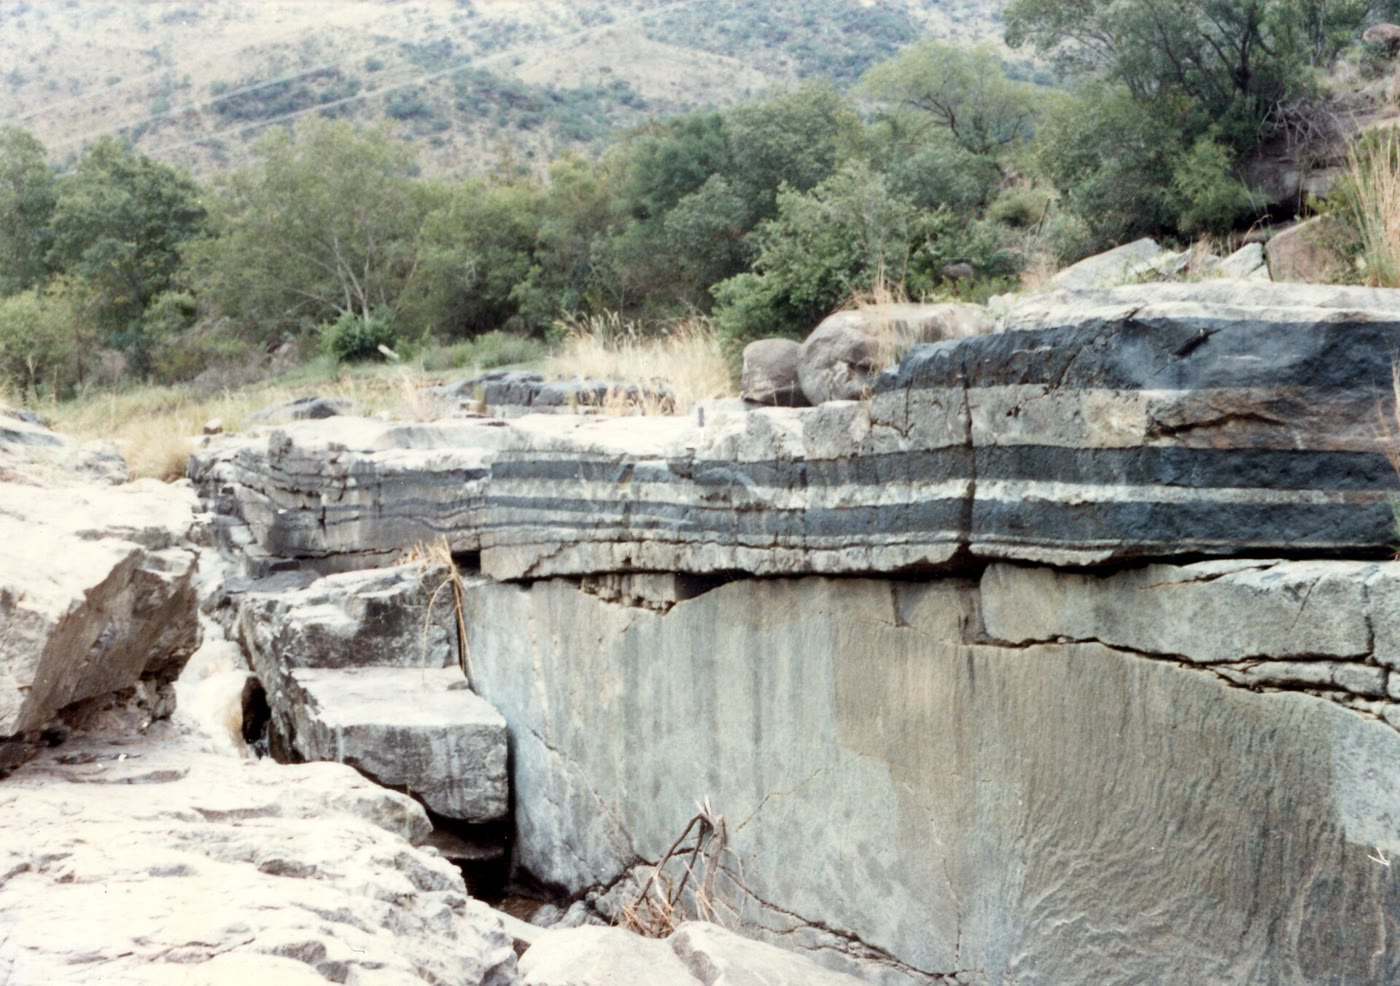
\includegraphics[height=5.2cm]{images/book4/b2-bushveld-chromitite.jpg}
\end{minipage}\hfill
\begin{minipage}[t]{0.42\linewidth}\vspace{0pt}\centering
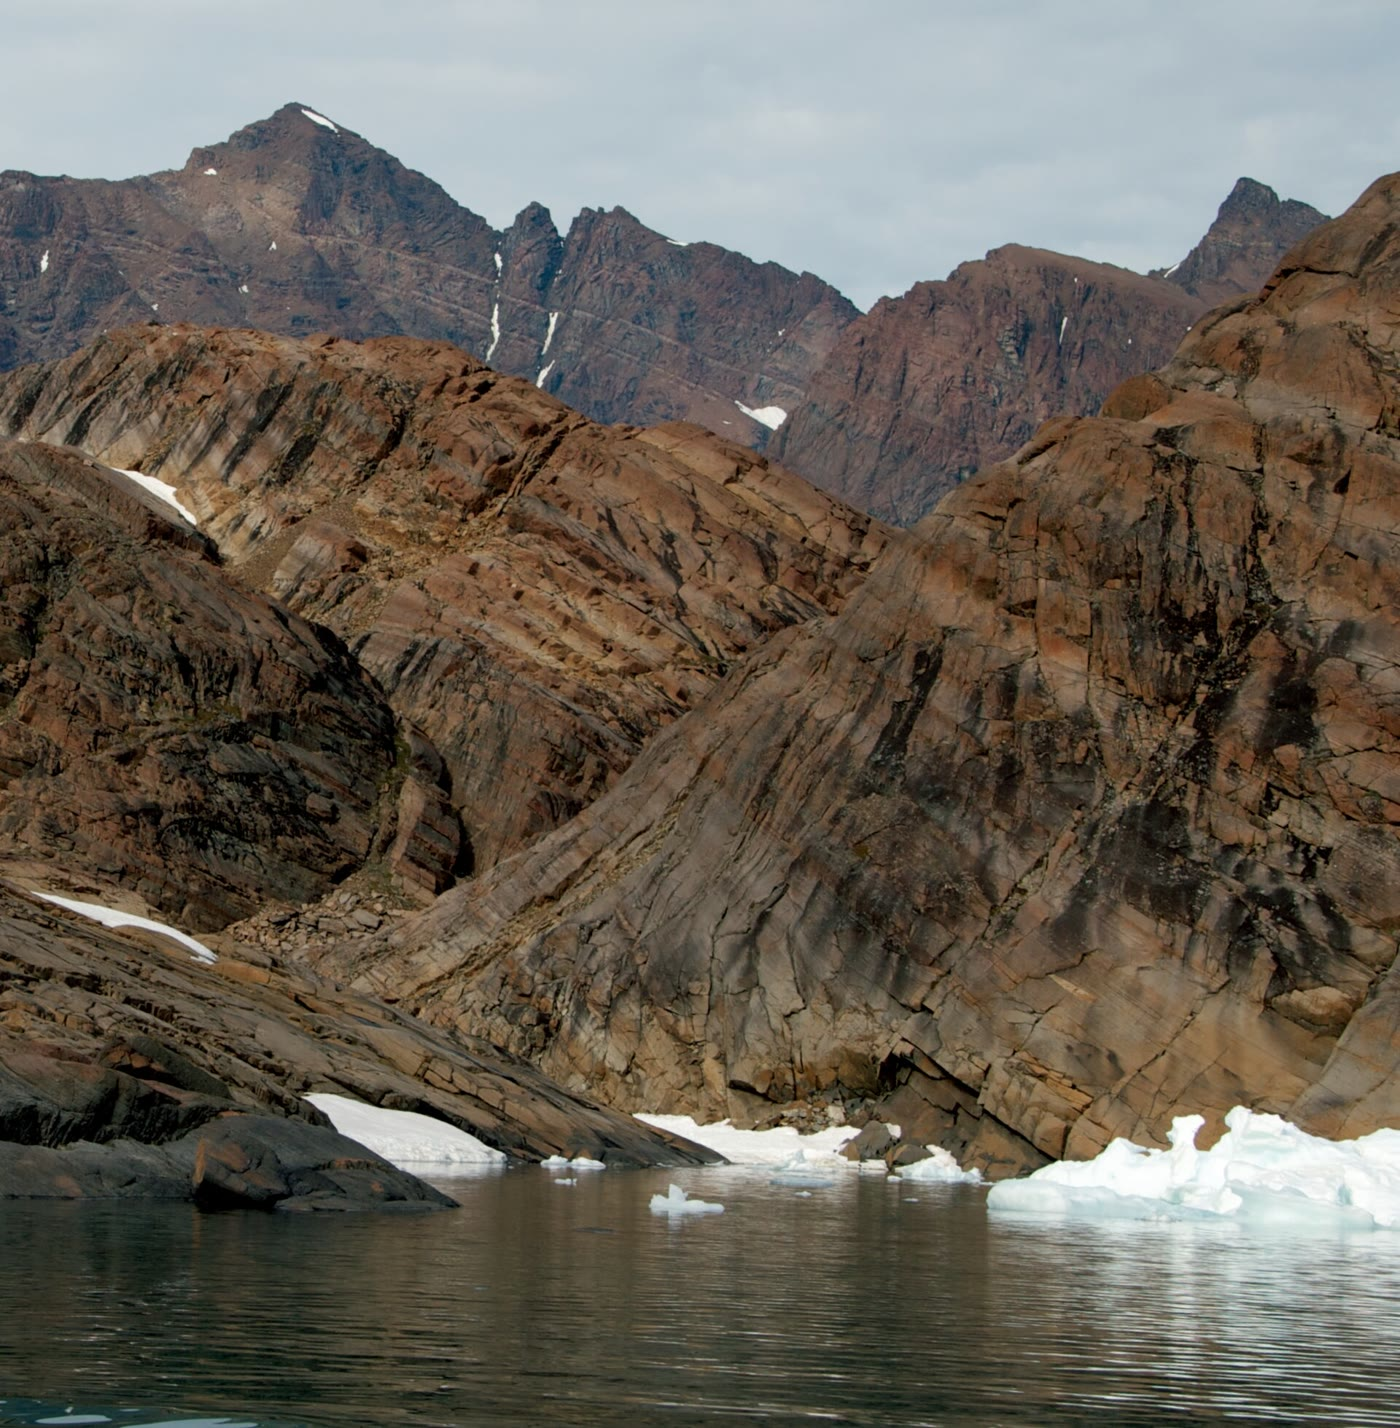
\includegraphics[height=5.2cm]{images/book4/b2-skaergaard-layering.jpg}
\end{minipage}
\par\smallskip{\small Izquierda: capas de cromitita negra y de anortosita gris de la
Zona Crítica del Complejo del Bushveld, Sudáfrica (Kevin Walsh, CC BY 2.0).
Derecha: los gabros estratificados de la Zona Media de la intrusión de Skaergaard, este de
Groenlandia, inclinados de arriba a la izquierda hacia abajo a la derecha (C. Tegner, CC BY 4.0).}
\end{omfigure}

\section{Sistemas abiertos}\label{sec:b2:magmatic-differentiation:open}

Una cámara magmática rara vez está cerrada. Llega \omterm{def:b2:magma-emplacement:magma}{magma} nuevo desde abajo, y las paredes de la
cámara son rocas que el \omterm{def:b2:magma-emplacement:magma}{magma} puede calentar, fundir y disolver.

\begin{definition}[Mezcla de magmas; asimilación cortical; AFC]
\label{def:b2:magmatic-differentiation:open}
La \emph{mezcla de magmas}\index{mezcla de magmas} es la combinación de dos \omterm{def:b2:magma-emplacement:magma}{magmas} de
composiciones distintas en uno solo. La \emph{asimilación cortical}\index{asimilación cortical} es la
incorporación de roca de la corteza a un \omterm{def:b2:magma-emplacement:magma}{magma}, por fusión y disolución de la roca
encajante o de bloques caídos en él. La \emph{asimilación con cristalización
fraccionada}\index{asimilación con cristalización fraccionada} (AFC) es su
combinación en una misma cámara: el \omterm{def:b2:magma-emplacement:magma}{magma} cristaliza, y el calor latente liberado
funde y asimila la roca encajante.
\end{definition}

\begin{proposition}[La mezcla es lineal en las concentraciones]\label{prop:b2:magmatic-differentiation:mixing}
Una mezcla de una fracción másica $s$ del \omterm{def:b2:magma-emplacement:magma}{magma} A y $1-s$ del \omterm{def:b2:magma-emplacement:magma}{magma} B tiene cada
concentración $C = sC_A + (1-s)C_B$: en cualquier diagrama de una concentración frente a
otra, las mezclas están sobre el segmento recto de A a B, y la regla de la palanca da
$s$.
\end{proposition}

\begin{proof}
Cada elemento se conserva: $C(m_A + m_B) = m_AC_A + m_BC_B$; divídase por $m_A + m_B$.
\end{proof}

La mezcla y la retirada de cristales trazan ambas rectas en los \omterm{def:b2:magmatic-differentiation:harker}{diagramas de Harker}; las razones
isotópicas las distinguen. La cristalización no cambia una razón isotópica, mientras que
la mezcla con una roca de razón distinta sí lo hace, a lo largo de la hipérbola del
\cref{ch:b2:isotope-geochemistry}. Un aumento de $^{87}$Sr/$^{86}$Sr con la sílice en una
serie volcánica es por tanto la huella de la asimilación.

\begin{proposition}[Asimilación con cristalización fraccionada]
\label{prop:b2:magmatic-differentiation:afc}
Un \omterm{def:b2:magma-emplacement:magma}{magma} cristaliza cristales con coeficiente de reparto global $D$ para un elemento
y asimila roca encajante de concentración $C_a$ a un ritmo $r$ veces el de
cristalización ($r \ne 1$). Con $F$ la masa de \omterm{def:b2:magma-emplacement:magma}{magma} relativa a su masa inicial
y $z = (r + D - 1)/(r - 1)$,
\[
\frac{C}{C_0} = F^{-z} + \frac{r}{r - 1 + D}\,\frac{C_a}{C_0}\,\bigl(1 - F^{-z}\bigr).
\]
Para $r = 0$ es la ley de Rayleigh. La razón isotópica del elemento en el \omterm{def:b2:magma-emplacement:magma}{magma}
es la media de la del \omterm{def:b2:magma-emplacement:magma}{magma} inicial y la de la roca encajante, ponderada por los
dos términos de esta suma.
\end{proposition}

\begin{proof}
Por unidad de masa inicial, cuando cristaliza una masa $\mathrm dm_c$, se asimila una masa
$r\,\mathrm dm_c$ y la masa del \omterm{def:b2:magma-emplacement:magma}{magma} cambia en $\mathrm dM =
-(1-r)\,\mathrm dm_c$. El balance del elemento es $\mathrm d(MC) = rC_a\,\mathrm dm_c -
DC\,\mathrm dm_c$. Desarrollando el miembro izquierdo y sustituyendo $\mathrm dm_c$ por
$-\mathrm dM/(1-r)$,
\[
M\frac{\mathrm dC}{\mathrm dM} = -C - \frac{rC_a - DC}{1-r}
= \frac{(r - 1 + D)\,C - rC_a}{1 - r} = -z\,\bigl(C - C^*\bigr),
\qquad C^* = \frac{rC_a}{r - 1 + D}.
\]
Así, $\mathrm d(C - C^*)/(C - C^*) = -z\,\mathrm dM/M$, y $C - C^*$ es proporcional
a $M^{-z}$; con $C = C_0$ en $M = 1$, $C = C^* + (C_0 - C^*)F^{-z}$, que es la
fórmula. Para $r = 0$, $z = 1 - D$ y $C^* = 0$. Los átomos que proceden del
\omterm{def:b2:magma-emplacement:magma}{magma} inicial obedecen la misma ecuación con $C_a = 0$, así que su concentración es
$C_0F^{-z}$; el resto procede de la pared: de ahí la ponderación de las razones isotópicas.
\end{proof}

DePaolo dio estas ecuaciones en 1981, y son el modelo estándar de un \omterm{def:b2:magma-emplacement:magma}{magma}
contaminado en su paso por la corteza. Esconden una restricción térmica. El calor
para asimilar roca procede del calor latente de los cristales: calentar corteza de
150 a \qty{1150}{\celsius} exige cerca de \qty{1}{kJ/g}, fundirla \qty{300}{J/g},
mientras que la cristalización del \omterm{def:b2:magma-emplacement:magma}{magma} aporta unos \qty{400}{J/g}; así que deben cristalizar unos \qty{3.25}{g} de
\omterm{def:b2:magma-emplacement:magma}{magma} por cada gramo de roca asimilada, y $r$ queda muy por debajo de 1.
Wilcox hizo el mismo cálculo para el Parícutin: sus \qty{25.4}{g} de monzonita
cuarcífera, tomados a unos \qty{200}{\celsius}, necesitaban unos \qty{31350}{J} para
calentarse hasta \qty{1100}{\celsius} y fundirse, el calor de cristalización de unos
\qty{85}{g} de plagioclasa, mucho más que los \qty{12.5}{g} de cristales que retiraba su balance
de masas. El \omterm{def:b2:magma-emplacement:magma}{magma} emitido no pudo pagar su propia asimilación:
el calor debió de proceder de un cuerpo de \omterm{def:b2:magma-emplacement:magma}{magma} mayor que el que entró en erupción,
que cristalizaba fuera de la vista (\cref{exo:b2:magmatic-differentiation:11}).
% ledger: depaolo81:afc, white09:afc-heat, wilcox54:heat, wilcox54:mass-balance

\begin{omfigure}
\centering
\begin{tikzpicture}
\begin{axis}[omrecord, name=left, width=0.47\linewidth, height=5.4cm,
  xmin=0.3, xmax=1, ymin=0.3, ymax=1.05, x dir=reverse,
  xlabel={magma restante $F$}, ylabel={Sr: $C/C_0$},
  tick label style={font=\scriptsize}, label style={font=\small}]
\addplot[thick, black] table[x=F, y=srC_r0] {figdata/out/bachelor-2-differentiation-afc.dat};
\addplot[thick, blue!70!black] table[x=F, y=srC_r02] {figdata/out/bachelor-2-differentiation-afc.dat};
\addplot[thick, red!70!black] table[x=F, y=srC_r05] {figdata/out/bachelor-2-differentiation-afc.dat};
\end{axis}
\begin{axis}[omrecord, at={(left.east)}, anchor=west, xshift=1.7cm,
  width=0.47\linewidth, height=5.4cm,
  xmin=0.3, xmax=1, ymin=0.703, ymax=0.716, x dir=reverse,
  xlabel={magma restante $F$}, ylabel={$^{87}$Sr/$^{86}$Sr},
  y tick label style={/pgf/number format/fixed, /pgf/number format/precision=3},
  legend style={font=\scriptsize, at={(0.03,0.97)}, anchor=north west},
  tick label style={font=\scriptsize}, label style={font=\small}]
\addplot[thick, black] table[x=F, y=iso_r0] {figdata/out/bachelor-2-differentiation-afc.dat};
\addlegendentry{$r = 0$}
\addplot[thick, blue!70!black] table[x=F, y=iso_r02] {figdata/out/bachelor-2-differentiation-afc.dat};
\addlegendentry{$r = 0.2$}
\addplot[thick, red!70!black] table[x=F, y=iso_r05] {figdata/out/bachelor-2-differentiation-afc.dat};
\addlegendentry{$r = 0.5$}
\end{axis}
\end{tikzpicture}
\par\smallskip{\small \omterm{def:b2:magmatic-differentiation:open}{Asimilación con cristalización fraccionada} para el estroncio
($D = 1.5$, roca encajante con la mitad del estroncio del \omterm{def:b2:magma-emplacement:magma}{magma} y
$^{87}$Sr/$^{86}$Sr = 0.7200, \omterm{def:b2:magma-emplacement:magma}{magma} 0.7035; valores ilustrativos). Izquierda: la
concentración baja más deprisa cuanto mayor es el ritmo de asimilación $r$, ya que la roca encajante aporta
menos estroncio y se forman más cristales para el mismo $F$. Derecha: la razón
isotópica, que la cristalización sola no cambia ($r = 0$), sube hacia la de la pared.}
\end{omfigure}

\section{Leer los cristales zonados}\label{sec:b2:magmatic-differentiation:zoning}

\begin{definition}[Zonación composicional]\label{def:b2:magmatic-differentiation:zoning}
Un cristal de una solución sólida presenta \emph{zonación composicional}\index{zonación composicional}
cuando su composición varía del núcleo al borde, registrando el líquido cambiante
a partir del cual crecieron las capas sucesivas. La zonación es \emph{normal} cuando el borde es más rico en
el componente de baja temperatura (el sodio en la plagioclasa), \emph{inversa} cuando es
más rico en el de alta temperatura, y \emph{oscilatoria} cuando alterna.
\end{definition}

Un cristal zonado es la \omterm{def:b2:magmatic-differentiation:crystallisation}{cristalización fraccionada} sorprendida en el acto: su núcleo no se
reequilibró con el líquido posterior. La figura siguiente calcula, sobre el bucle de Bowen,
la plagioclasa que crece de un líquido con un \qty{50}{\percent} de anortita. En
equilibrio los cristales siguen siendo homogéneos y terminan en un \qty{50}{\percent}; en una \omterm{def:b2:magmatic-differentiation:crystallisation}{cristalización
fraccionada} perfecta cada capa nueva está en equilibrio con un líquido cada vez más sódico,
y el borde de los últimos cristales es albita casi pura. La zonación normal, de
núcleo cálcico a borde sódico, es lo que predice la serie de Bowen para un \omterm{def:b2:magma-emplacement:magma}{magma} que se enfría. Una zona
inversa, una banda cálcica por fuera de una sódica, dice que el cristal quedó bañado de repente en
un líquido más caliente o más cálcico: a menudo la llegada de \omterm{def:b2:magma-emplacement:magma}{magma} nuevo, una mezcla en la
cámara.
% ledger: bowen13:plagioclase, earle:bowen (Book 2)

\begin{omfigure}
\centering
\begin{tikzpicture}
\begin{axis}[omrecord, width=0.78\linewidth, height=6cm,
  xmin=0, xmax=1, ymin=0, ymax=90,
  xlabel={fracción del líquido cristalizada},
  ylabel={anortita (\unit{\percent} molar)},
  legend style={font=\scriptsize, at={(0.02,0.02)}, anchor=south west},
  tick label style={font=\scriptsize}, label style={font=\small}]
\addplot[very thick, red!70!black] table[x=x, y=an_frac] {figdata/out/bachelor-2-differentiation-zoning.dat};
\addlegendentry{fraccionada: capa que se forma}
\addplot[thick, gray, densely dotted] table[x=x, y=an_liq_frac] {figdata/out/bachelor-2-differentiation-zoning.dat};
\addlegendentry{fraccionada: líquido}
\addplot[very thick, blue!70!black, dashed] table[x=x, y=an_eq] {figdata/out/bachelor-2-differentiation-zoning.dat};
\addlegendentry{equilibrio: cristales}
\end{axis}
\end{tikzpicture}
\par\smallskip{\small Plagioclasa que cristaliza de un líquido con un \qty{50}{\percent} de
anortita, calculada sobre el bucle de Bowen (1913). En la \omterm{def:b2:magmatic-differentiation:crystallisation}{cristalización fraccionada} las
capas sucesivas de los cristales, del núcleo (izquierda) al borde (derecha), son cada vez más
sódicas, y el líquido alcanza la albita cuando ha cristalizado cerca de un \qty{82}{\percent}; en la
\omterm{def:b2:magmatic-differentiation:crystallisation}{cristalización en equilibrio} los cristales permanecen uniformes y terminan con la composición del
líquido del que proceden.}
\end{omfigure}

\begin{inthelab}[Leer los cristales zonados]
Los petrólogos leen primero la zonación con polarizadores cruzados, donde las zonas de una
plagioclasa se extinguen con ángulos ligeramente distintos y aparecen como bandas concéntricas.
Después la miden: una microsonda electrónica (\cref{ch:b2:field-lab-methods-2})
analiza puntos de unos pocos micrómetros a lo largo de un perfil del núcleo al borde, y los mapas
de calcio y sodio muestran las zonas directamente. A partir de ese perfil calculan la
composición del líquido del que creció cada zona, con el bucle de la figura anterior o
con coeficientes de reparto, y cuentan las zonas inversas como el número de
recargas de la cámara. Los \omterm{def:b2:elements-in-the-earth:trace}{elementos en trazas} medidos a lo largo del mismo perfil por ablación
láser, y las razones isotópicas medidas zona a zona, separan la cristalización, la mezcla
y la asimilación en la historia de un solo cristal.
\end{inthelab}

\section{Ejercicios}

\begin{exercise}[$\star$]\label{exo:b2:magmatic-differentiation:1}
Úsense las medidas de Bowen sobre las plagioclasas (solidus / liquidus, \unit{\celsius}):
An$_{100}$ 1550 / 1550; An$_{83.3}$ 1465 / 1521; An$_{66.7}$ 1372 / 1490; An$_{50}$
1287 / 1450; An$_{33.3}$ 1205 / 1394; An$_{20}$ liquidus 1334; An$_{11.1}$ liquidus
1265, e interpólese linealmente entre puntos vecinos. Un líquido con un
\qty{50}{\percent} de anortita se enfría en equilibrio. (a) ¿A qué temperatura
empieza a cristalizar, y cuál es la composición del primer cristal? (b) A
\qty{1394}{\celsius}, ¿cuáles son las composiciones del líquido y de los cristales,
y qué fracción másica ha cristalizado (úsense las fracciones molares como si fueran fracciones
másicas)? (c) ¿Cuál es la composición de la última gota de líquido?
\end{exercise}
% ledger: bowen13:plagioclase

\begin{exercise}[$\star$]\label{exo:b2:magmatic-differentiation:2}
Un \omterm{def:b2:magmatic-differentiation:cumulate}{cumulado} gabroico contiene un \qty{50}{\percent} de plagioclasa, un \qty{35}{\percent} de
clinopiroxeno y un \qty{15}{\percent} de olivino. Con los coeficientes de reparto
(olivino / clinopiroxeno / plagioclasa) Sr 0.000063 / 0.157 / 2.7, Zr 0.00068 /
0.195 / 0.001 y Rb 0.000044 / 0.0033 / 0.025, calcúlese el coeficiente de reparto
global de cada elemento, y dígase cuál es compatible.
\end{exercise}
% ledger: white07:kd-basalt

\begin{exercise}[$\star$]\label{exo:b2:magmatic-differentiation:3}
El \omterm{def:b2:magmatic-differentiation:cumulate}{cumulado} del \cref{exo:b2:magmatic-differentiation:2} cristaliza a partir de un basalto, por \omterm{def:b2:magmatic-differentiation:crystallisation}{cristalización fraccionada},
hasta que queda la mitad del líquido. (a) ¿En qué factor ha cambiado cada uno de Sr, Zr y Rb
en el líquido (tómense los coeficientes globales 1.40, 0.069 y 0.014)? (b) ¿En qué factor
ha cambiado la razón Zr/Rb? Coméntese con el corolario sobre las razones.
\end{exercise}
% ledger: white07:kd-basalt

\begin{exercise}[$\star$]\label{exo:b2:magmatic-differentiation:4}
La primera lava del Parícutin (febrero de 1943) tenía un \qty{55.04}{\percent} de \ce{SiO2},
un \qty{5.68}{\percent} de \ce{MgO} y un \qty{0.85}{\percent} de \ce{K2O}; la última (febrero de
1952), 60.07, 3.73 y \qty{1.67}{\percent}. (a) Calcúlese el cambio de cada óxido.
(b) La potasa no entra en ninguno de los minerales que cristalizan. Si se hubiera concentrado solo por
\omterm{def:b2:magmatic-differentiation:crystallisation}{cristalización fraccionada}, ¿qué fracción del líquido habría quedado?
(c) El balance de masas de Wilcox solo retira unos \qty{12.5}{g} de cristales por cada
\qty{100}{g} de \omterm{def:b2:magma-emplacement:magma}{magma}. ¿Qué sugiere la comparación?
\end{exercise}
% ledger: wilcox54:table2, wilcox54:mass-balance

\begin{exercise}[$\star\star$]\label{exo:b2:magmatic-differentiation:5}
Compárense la \omterm{def:b2:magmatic-differentiation:crystallisation}{cristalización fraccionada} y la \omterm{def:b2:magmatic-differentiation:crystallisation}{cristalización en equilibrio}: calcúlese $C_L/C_0$ con ambas leyes
(a) para el níquel, $D = 5$, cuando ha cristalizado un \qty{20}{\percent} del líquido; (b)
para un \omterm{def:b2:elements-in-the-earth:partition}{elemento incompatible}, $D = 0.01$, cuando ha cristalizado un \qty{90}{\percent}.
(c) ¿Cuáles son los límites de ambas leyes cuando $F \to 0$? ¿Qué ley puede despojar a un líquido de un
\omterm{def:b2:elements-in-the-earth:partition}{elemento compatible} por completo?
\end{exercise}

\begin{exercise}[$\star\star$]\label{exo:b2:magmatic-differentiation:6}
(a) Calcúlense los porcentajes en masa de \ce{MgO}, \ce{FeO} y \ce{SiO2} en el olivino
Fo$_{80}$, $(\ce{Mg}_{0.8}\ce{Fe}_{0.2})_2\ce{SiO4}$ ($M$ = 40.30, 71.84 y
\qty{60.08}{g/mol}). (b) Un basalto con un \qty{10.0}{\percent} de \ce{MgO} y un
\qty{49.0}{\percent} de \ce{SiO2} cristaliza solo este olivino hasta que su líquido tiene un
\qty{8.0}{\percent} de \ce{MgO}. ¿Qué fracción másica de olivino se retiró? (c) ¿Cuál
es entonces el contenido en sílice del líquido?
\end{exercise}

\begin{exercise}[$\star\star$]\label{exo:b2:magmatic-differentiation:7}
Para la intrusión de Skaergaard, $F = \num{1.091e-7}H^2 - \num{5.9064e-4}H + 0.7678$.
(a) Calcúlese $F$ en $H = 0$, 1000 y \qty{2000}{m}. (b) ¿A qué altura es $F = 0$?
(c) ¿Qué fracción del \omterm{def:b2:magma-emplacement:magma}{magma} había cristalizado antes de que se formara la base de la secuencia
aflorante del suelo, y dónde podría estar?
\end{exercise}
% ledger: tegner23:skaergaard

\begin{exercise}[$\star\star$]\label{exo:b2:magmatic-differentiation:8}
A lo largo de la sección de Skaergaard, el \omterm{def:b2:magmatic-differentiation:cumulate}{cumulado} mediano contiene \qty{177}{ppm} de Ni en
$F = 0.70$ (Zona Inferior a), \qty{54}{ppm} en $F = 0.29$ (Zona Media) y
\qty{6.2}{ppm} en $F = 0.17$ (Zona Superior a). (a) Suponiendo que los \omterm{def:b2:magmatic-differentiation:cumulate}{cumulados} contienen
$D$ veces el níquel de su líquido y que el líquido sigue la ley de Rayleigh,
calcúlese el $D$ aparente entre los dos primeros niveles. (b) Hágase lo mismo entre los
dos últimos. (c) ¿Qué puede hacer cambiar el $D$ aparente?
\end{exercise}
% ledger: data:b4-skaergaard

\begin{exercise}[$\star\star$]\label{exo:b2:magmatic-differentiation:9}
Compruébese la respuesta de Wilcox: \qty{100}{g} de pasta de la primera lava (\ce{SiO2}
55.53, \ce{MgO} 4.66, \ce{K2O} \qty{0.88}{\percent}) más \qty{25.4}{g} del xenolito
medio (72.48, 0.77, 3.64) menos \qty{2.9}{g} de olivino Fo$_{80}$ (39.19, 42.06, 0)
menos \qty{9.6}{g} de plagioclasa An$_{70}$ (50.54, 0, 0). (a) ¿Qué masa queda?
(b) Calcúlense sus \ce{SiO2}, \ce{MgO} y \ce{K2O} y compárense con la pasta de la
lava 19 (60.16, 3.19 y \qty{1.75}{\percent}). (c) ¿Qué óxido se ajusta peor?
\end{exercise}
% ledger: wilcox54:groundmass, wilcox54:xenoliths, wilcox54:mass-balance

\begin{exercise}[$\star\star\star$]\label{exo:b2:magmatic-differentiation:10}
Un \omterm{def:b2:magma-emplacement:magma}{magma} asimila roca encajante con $r = 0.2$ mientras cristaliza, con $D_{\ce{Sr}} =
1.5$, $C_a/C_0 = 0.5$, $^{87}$Sr/$^{86}$Sr inicial = 0.7035 y roca encajante 0.7200.
(a) Calcúlense $z$, $F^{-z}$ y $C/C_0$ en $F = 0.7$. (b) Compárese con la \omterm{def:b2:magmatic-differentiation:crystallisation}{cristalización
fraccionada} pura con el mismo $F$, y explíquese la diferencia con la masa de cristales
formada en cada caso. (c) Calcúlese la $^{87}$Sr/$^{86}$Sr del \omterm{def:b2:magma-emplacement:magma}{magma}.
\end{exercise}

\begin{exercise}[$\star\star\star$]\label{exo:b2:magmatic-differentiation:11}
Sígase el balance térmico de Wilcox para el Parícutin. (a) ¿Cuánto calor necesita un gramo de monzonita
cuarcífera para pasar de 200 a \qty{1100}{\celsius} (capacidad calorífica
\qty{1.1}{J/(g.K)}) y después fundirse (\qty{250}{J/g})? (b) ¿Cuánto para
\qty{25.4}{g}? (c) ¿Qué masa de plagioclasa An$_{70}$ (calor latente \qty{370}{J/g})
debe cristalizar para aportarlo? (d) Compárese con los \qty{12.5}{g} de cristales del
balance de masas, calcúlese la razón $r$ entre asimilación y cristalización, y dígase qué
implica.
\end{exercise}
% ledger: wilcox54:heat, white09:afc-heat

\begin{exercise}[$\star\star\star$]\label{exo:b2:magmatic-differentiation:12}
Un basalto con \qty{250}{ppm} de Ni cristaliza primero olivino solo ($D = 5$) hasta
$F = 0.8$, y después olivino con plagioclasa y clinopiroxeno ($D = 1.5$ global). (a)
Calcúlese el factor en que cambia el níquel en cada etapa, y el contenido en níquel del
líquido en $F = 0.5$. (b) ¿Qué habría predicho una única ley con $D = 5$?
(c) Explíquese por qué la ley de Rayleigh debe aplicarse por etapas.
\end{exercise}

\section{Problema: la intrusión que escribió su propia historia}

\begin{problem}[{Problema de fin de semana --- de las capas de un gabro a la fracción de
su magma que seguía líquida al final}]
\label{pb:b2:magmatic-differentiation:1}
Un sill de gabro estratificado (inventado) cristalizó a partir de un basalto cuyo borde enfriado
da la composición parental: \ce{SiO2} 49.5, \ce{Al2O3} 16.0, \ce{FeO} 10.0,
\ce{MgO} 9.0, \ce{CaO} 11.5, \ce{Na2O} 2.5, \ce{K2O} \qty{0.30}{\percent};
\qty{150}{ppm} de Ni y \qty{80}{ppm} de Zr. Los \omterm{def:b2:magmatic-differentiation:cumulate}{cumulados} de la zona inferior constan de un
\qty{20}{\percent} de olivino, un \qty{50}{\percent} de plagioclasa y un \qty{30}{\percent} de
clinopiroxeno; por encima del nivel donde desaparece el olivino, de un \qty{55}{\percent} de
plagioclasa y un \qty{45}{\percent} de clinopiroxeno. Tómense los coeficientes de reparto
(olivino / plagioclasa / clinopiroxeno) Ni 5.0 / 0 / 2.0 y Zr 0.0007 / 0.001 /
0.195. Composiciones de los minerales (\unit{\percent}): olivino \ce{MgO} 42.06, \ce{CaO} 0,
\ce{Al2O3} 0, \ce{SiO2} 39.19; plagioclasa 0, 14.36, 31.70, 50.54; clinopiroxeno
16.0, 20.5, 3.0, 51.5. Un \omterm{def:b2:magma-emplacement:bodies}{dique}
de roca de grano fino alimentado desde la cámara cuando cristalizó la capa más alta tiene
\ce{SiO2} 50.0, \ce{Al2O3} 14.1, \ce{FeO} 16.7, \ce{MgO} 4.9, \ce{CaO} 7.3,
\ce{Na2O} 3.4, \ce{K2O} \qty{0.75}{\percent} y \qty{188}{ppm} de Zr.

\noindent\textbf{Parte I --- Los coeficientes de reparto de las capas.}
\begin{enumerate}
\item Calcúlese el coeficiente de reparto global del níquel en la zona inferior.
\item Calcúlese el del circonio en la zona inferior.
\item Calcúlense ambos en la zona superior.
\item ¿Qué elemento es compatible en cada zona? ¿Sigue siendo compatible el níquel cuando
desaparece el olivino?
\item ¿Qué mineral contiene la mayor parte del circonio de los \omterm{def:b2:magmatic-differentiation:cumulate}{cumulados}, y por qué?
\item ¿En qué factor cambia Ni/Zr en el líquido cada vez que $F$ se reduce a la mitad en la zona
inferior?
\end{enumerate}

\noindent\textbf{Parte II --- Curvas de Rayleigh a lo largo de la sección.}
\begin{enumerate}[resume]
\item ¿Qué contenido en níquel se espera en el \omterm{def:b2:magmatic-differentiation:cumulate}{cumulado} más bajo, cristalizado en
$F = 1$?
\item Un \omterm{def:b2:magmatic-differentiation:cumulate}{cumulado} de la zona inferior situado más arriba contiene \qty{190}{ppm} de Ni. ¿Con qué $F$ se
formó?
\item ¿Cuál era entonces el contenido en circonio del líquido?
\item Con ese $F$, compárese el níquel del líquido dado por la ley fraccionada y por la
ley de equilibrio.
\item El olivino desaparece en $F = 0.55$. Calcúlese el contenido en níquel del líquido
en ese punto.
\item Calcúlese el níquel de los \omterm{def:b2:magmatic-differentiation:cumulate}{cumulados} formados justo por debajo y justo por encima de ese
nivel. ¿Qué rasgo vería un geólogo en el perfil?
\item Calcúlese el níquel del líquido y del \omterm{def:b2:magmatic-differentiation:cumulate}{cumulado} en $F = 0.40$. Explíquese
la tendencia.
\end{enumerate}

\noindent\textbf{Parte III --- El balance de masas del último líquido.}
\begin{enumerate}[resume]
\item Escríbase la ecuación de conservación del método para un óxido, con las masas
$x_{\mathrm{ol}}, x_{\mathrm{pl}}, x_{\mathrm{cpx}}$ retiradas por cada \qty{100}{g} de
\omterm{def:b2:magma-emplacement:magma}{magma} parental y el \omterm{def:b2:magma-emplacement:bodies}{dique} como líquido hijo.
\item Escríbase para \ce{MgO}, \ce{CaO} y \ce{Al2O3}.
\item Resuélvase el sistema $3 \times 3$.
\item ¿Qué fracción del \omterm{def:b2:magma-emplacement:magma}{magma} parental queda como líquido?
\item Compruébese la respuesta con \ce{SiO2}: recalcúlese la sílice del líquido a partir de las
masas halladas.
\item Compárense las proporciones de los minerales retirados con las modas de las dos
zonas.
\item La potasa no entra en ninguno de los minerales: ¿qué fracción de líquido da?
\end{enumerate}

\noindent\textbf{Parte IV --- La fracción de líquido en la cima.}
\begin{enumerate}[resume]
\item ¿En qué factor había aumentado el circonio en el líquido cuando el olivino desapareció en
$F = 0.55$? Dese entonces el contenido en circonio.
\item A partir del circonio del \omterm{def:b2:magma-emplacement:bodies}{dique}, calcúlese la fracción de líquido restante cuando
se formó, aplicando la ley de la zona superior desde $F = 0.55$.
\item Rehágase el cálculo con un único $D = 0.07$ desde el principio. ¿Es sensible la respuesta
a los detalles de $D$?
\item El hierro pasó de un 10.0 a un \qty{16.7}{\percent} en el líquido mientras la sílice apenas
cambiaba. ¿Qué minerales son responsables, y qué tipo de serie magmática
anuncia esto (\cref{ch:b2:magmatic-series})?
\item Los \omterm{def:b2:magmatic-differentiation:cumulate}{cumulados} más altos contienen \qty{47}{ppm} de Zr. Los cristales cúmulo solos contendrían
$\bar D$ veces el circonio del líquido; ¿qué fracción másica de líquido atrapado
(con la composición del \omterm{def:b2:magma-emplacement:bodies}{dique}) explica el análisis?
\item Dese la fracción del \omterm{def:b2:magma-emplacement:magma}{magma} original que seguía líquida cuando cristalizó la capa más
alta, el número clave de este problema, y compárense las tres estimaciones
(elementos mayores, potasa, circonio).
\end{enumerate}
\end{problem}
% ledger: white07:kd-basalt, matzen12:dni
